%!TEX root = ../../thesis.tex
\section{History of soft robotics: what are they?} 
\label{sec:intro:history}
% https://cyberneticzoo.com/bionics/1957-artificial-muscle-joseph-laws-mckibben-american/
The term \emph{soft robotics} is the abbreviated form of \emph{soft material robotics}. Although the words \emph{soft} and \emph{robotics} have a clear definitions independently, the collocation of the two has sparked vivid discussions and new idealogies within the robotics community for the past decades. %resulting in a dig touching the territories of the philosophical. 
Consequently, the exponentially increasing scientific interest in soft robotics that boomed in the early 2010s, which may be seen as a historical cornerstone that has revolutionized our perspective on the branching field of robotics as a whole. %and rekindled its original ambition even before the term \emph{robot} was introduced. 
Although the debate on its exact terminology is still ongoing, and perhaps may never be closed; we will discuss its rich history and propose a terminologies for \emph{soft robotics} and related topics in the field based an ensemble of prior literature. Naturally, the terms used in this thesis might deviate from literature, but are perhaps necessary to avoid disambiguity with this multidisciplinary topic. Let us introduce the following:
%
\terminology{\textbf{Soft robotics} is a robotics subclass with purposefully designed compliant elements embedded into their mechanical structure whose goal is to endow the robot with natural (or biological) motion or compliance.}{}
%
The definition above is adopted from the work of Della Santina et al. \cite{}, yet modified to highlight the importance of soft materials to mimic biological motion -- also referred to as \emph{bio-mimicry}. The ambition of closely mimicking biological creatures is perhaps not commonly associated with the field of robotics, given its importance in automation industry, yet the inception of robotics can originally be found in bio-mimicry when regarding its rich history. We would like to invite the reader to embark with us a brief section into a short history of (soft) robotics. Hereby showing that the current trends of bio-mimicry and soft robotics find roots in a periods way before its academic boom in the early 2010's.
\vspace{0.085em}
%
\afterpage{
\begin{figure}
\hspace{-7mm}
\includegraphics[width=1.11\textwidth]{./3_chapters/0_introduction/img/timeline_printer.pdf}
\caption{A brief timeline of the state-of-the-art of bio-inspired robotics throughout human history. {(420 BC)} One of the earliest examples of bio-mimicry -- the flying mechanical bird. {(1495)} The Mechanical Knight by Leonardo Da Vinci. {(1954)} Unimate, the first industrial robot. {(1957)} McKibben actuator, an early soft actuator inspired by the human muscle used for rehabilitation purposes. {(1965)} Orm, the first soft robotic system designed by V. Scheinman and L. Leifer. {(1981)} Canadarm-1, early flexibile robotics employed on the International Space Station (ISS). {(1989)} The soft robotic gripper developed by Suzumori et al. (1989, \cite{Suzumori1991}), seen as one of the earliest \textit{academic} soft robot, developed before the word \emph{soft robot} existed. {(2010)} Festo's Bionic arm inspired by the elephant's trunk. (2012) Multi-gait soft robot capable of terrestial locomotion \cite{Choi2011}. (2016) Octo-bot, the first full autonomous 3D-printed soft robot that explores a stabilizing oscillator chemical network that produces preprogrammed repetitive motion \cite{Wehner2016}
}
\end{figure}
\clearpage
}

\textbf{(Biomimicry in early automata)} One of the earliest examples of bio-mimicry is a mechanical wooden dove developed by mathematician Archytas of Tarentum in 350 BC. According to historians, the system was driven by compressed air or an internal steam-driven engine to achieve forward propulsion. It was believed to achieve traveling distances of ~200 \si{\meter} (see note\footnote{It was unclear if the devices was attached to a rope, or autonomous flight was achieved.}). Although might argue its lacks to sophistication to be considered a \emph{robot}, Archytas's invention could be considered as one of the earliest robotic aviation, as its mechanical principles of achieving motion are undoubtedly similar to nowadays \emph{drone} technology. A millennium later, in the period of the High Renaissance, Leonardo da Vinci designed and constructed a mechanical knight around the 1490's -- and is thought to be the earliest robotic system. The mechanical constructions are perhaps closer to classical robots given our current perspective, and it was capable of various complex motions using preprogrammed sequences. It is well-known that his work was built upon extensive anatomical research, which may have facilitated a deep understanding of the human body into the mechanical knight's robotic design. Given the work of Archytas and Da Vinci, biomimicry played a paramount role in the development of robot technologies before the term \emph{robot} was even introduced.

%\par In the 1920's, shortly after the second industrial revolution (1870 - 1914) and the first world war (1914), the first usage of the work \emph{robot} appeared -- originally meaning 'forced labor by serfs' (\ie, peasants) derived from the Czech word \emph{robota}. An common misconception is that robot implies slave, nonetheless, its origin is somewhat related. The word was popularized by Karel \v{C}apek in his play R.U.R. (Rossum’s Universal Robots) that involves an inventor named Rossum who discovers the secret of creating human-like machines. In his play, Rossom's robots assisted or fully alleviated mankind from any labor. Through human's ambition to assimilate man and machine, the robots ultimately gained the capacity for emotions. Shortly after, the robots, who were created to serve humans, have come to dominate mankind completely. The word \emph{robotics} was later solidified by Isaac Asimov, adapting the term from \v{C}apek. These works of science fiction are perhaps the fundamental groundwork of modern robotics which have led to the base practices of robotics and its corresponding academic field.

Three decades later, in 1954, George Devol filed a patent describing an autonomous robotic machine that could be preprogrammed to execute step-by-step motions \cite{Mickle2008}. The machine was designed to reduce the workload on the manufacturing work floor, with a major focus on mimicking repetive human tasks. A robot was prototyped in 1958 under the name \emph{Unimate}. By 1961, the Unimate series became the first mass produced robotic arm for factory automation. The Unimate was used for manipulating metal die-casts and welding these to welding these to the main body of automobiles. In doing so revolutionizing the car industry shortly after. After its production, Devol and his partner Joseph Engelberger started a company called \emph{Unimation} in 1962. 
%Although revolutionary for its time, and shaped the perspective on benefits of robotics, the word \emph{robot} was already introduced 30 years earlier by Karel \v{C}apek, before the word \emph{robotics} was coined by Isaac Asimov in his book \textit{I, Robot} (1951). 
Interestingly, the Unimate explored both electric as hydraulic-mechanical actuation, a practice we see in nowadays very similar Atlas robot humanoid (2013) from company Boston Dynamics. Note that the robot were still controlled remotely, and rudimentary low-level controllers were applied then. Much later (1969), Victor Scheinman (student at the time) created the Stanford Arm, recognized as the first electronic computer-controlled robotic arm because the Unimate's instructions were stored on a magnetic drum. He ultimately developed the PUMA robot in 1972 -- the successor of the Unimate -- during his employment at Unimation. Please keep Scheinman in mind. \vspace{0.085em}

(\textbf{Early robotics with flexibility}) The early 1950's also brought forth the McKibben actuators developed by Joseph Laws McKibben (1957) -- a well-known work in the field of soft robotics. Surisingly, these actuators were developed three years after the release of the Unimate series. The McKibben actuator consisted of an inflatable inner bladder enveloped with a double-helical weave. When pressurized, the fluidic actuator converted radial expansion into uni-axial contraction since weave inhibited extensive \emph{ballooning} -- a term for undesired rapidly-accelerated volumetric expansion. A schematic representation of the McKibben actuator and the effect of ballooning are shown in Figure \ref{fig:C0:mckibben}. In modern soft robotics, ballooning is an (often undesired)nonlinear effect where the hyper-elastic pressure vessel exhibits strain-softening after a critical point is reached. As a result, further increase of the pressure leads to an exponential growth in volume, which ultimately leads to actuator tearing. At the stage of ballooning, mechanical performance significantly drops and even produces adverse effects, like actuator reversal. McKibben solve this problem using a combination of soft and inextensible materials.

The McKibben actuators are perhaps one of the first fundamental technologies that enabled soft robotics and to this day it remains a framework for many soft artificial muscle. Nevertheless, besides fluidics, there exist many other technologies employed in soft robotic motion that predate the invention of the McKibben actuator: such as thermal or chemical expansion/contraction, crystal re-alignment, di-electric elastomers, magnetism, and naturally electro-mechanical actuation. An early example of popular actuation techniques in soft robotics is the Dielectric Elastomer Actuators (DEA) developed by Wilhelm R\"{o}ntgen in 1880. Although such system are not categorized as soft robots, they are; however, categorized as soft actuators. We like to emphasize here the difference between soft actuators and soft robots in view of a terminology relevant to the thesis:

\terminology{\textbf{Soft actuators} are controllable flexible actuation units of the constitutive soft robotic system that through external stimuli allow for motion, or change in compliance and/or texture.}{}
%
%
\noindent The terminology above attempts to address a common ambiguity in soft robotics, that being interchangeably use of the word soft actuator and soft robot. Let us also introduce the dual of soft actuators -- namely the \emph{soft sensor} that relate measurements to the motion of soft actuators:
%
\begin{figure}[!t]
  %\hspace*{-1mm}
  \ifx\printFigures\undefined
  \else
  \centering
  % This file was created by matlab2tikz.
%
%The latest updates can be retrieved from
%  http://www.mathworks.com/matlabcentral/fileexchange/22022-matlab2tikz-matlab2tikz
%where you can also make suggestions and rate matlab2tikz.
%
\definecolor{mycolor1}{rgb}{0.06275,0.35686,0.84706}%
\definecolor{mycolor2}{rgb}{0.86667,0.21176,0.10980}%
%
\begin{tikzpicture}

\begin{axis}[%
width=0.602\textwidth,
height=0.161\textwidth,
at={(0\textwidth,0.015\textwidth)},
scale only axis,
axis on top,
xmin=0.5,
xmax=2426.5,
tick align=outside,
y dir=reverse,
ymin=0.5,
ymax=650.5,
axis line style={draw=none},
ticks=none
]
\addplot [forget plot] graphics [xmin=0.5, xmax=2426.5, ymin=0.5, ymax=650.5] {fig_1_1-1.png};
\end{axis}

\begin{axis}[%
width=0.302\textwidth,
height=0.191\textwidth,
at={(0.648\textwidth,0\textwidth)},
scale only axis,
xmin=0,
xmax=1.5,
xlabel style={font=\color{white!15!black}},
xlabel={pressure (kPa)},
ymin=0,
ymax=35,
axis background/.style={fill=white},
xmajorgrids,
ymajorgrids,
legend style={at={(0.03,0.97)}, anchor=north west, legend columns=2, legend cell align=left, align=left, draw=white!15!black}
]
\addplot [color=mycolor1, line width=1.5pt]
  table[row sep=crcr]{%
0	0\\
0.00600149999999999	3.0568983103671\\
0.012003	5.35826739157104\\
0.024006	7.86017230302163\\
0.036009	9.05072762147565\\
0.0480119999999999	9.795136933107\\
0.0600149999999999	10.3164705929212\\
0.0720179999999999	10.711316657325\\
0.0840209999999999	11.0279129564825\\
0.0960239999999999	11.2925201532359\\
0.108027	11.5206742947192\\
0.1260315	11.8150953044601\\
0.144036	12.0694590939099\\
0.1620405	12.2959065095095\\
0.1860465	12.5672572998435\\
0.2100525	12.8138561366798\\
0.24006	13.0980192458931\\
0.276069	13.4149916949781\\
0.3180795	13.7633415653589\\
0.372093	14.1910487738014\\
0.456113999999999	14.8357726162343\\
0.588146999999999	15.8481229823956\\
0.660164999999999	16.4166289214781\\
0.726181499999999	16.9548047718235\\
0.786196499999999	17.4617841353458\\
0.840209999999999	17.9350495132933\\
0.894223499999999	18.4266813211065\\
0.948236999999999	18.9389704257632\\
0.996248999999999	19.413653689242\\
1.044261	19.9084481551956\\
1.092273	20.4253835409611\\
1.140285	20.9666992209241\\
1.1822955	21.4623032550621\\
1.224306	21.9803397018051\\
1.2663165	22.5228818415618\\
1.308327	23.0922527983715\\
1.3503375	23.6910711317645\\
1.392348	24.322306181775\\
1.43435850000001	24.9893459441392\\
1.47036750000001	25.5925254860443\\
1.4999985	26.11365092975\\
};
\addlegendentry{$\delta V$}

\addplot [color=mycolor2, line width=1.5pt]
  table[row sep=crcr]{%
0	0\\
0.00600149999999999	0.57694322540025\\
0.012003	1.8809393408942\\
0.0180045	2.95152432065056\\
0.024006	4.45583458122557\\
0.036009	6.19378149929854\\
0.0480119999999999	7.48539157943733\\
0.0600149999999999	8.4688855095399\\
0.0720179999999999	9.23690647886306\\
0.0840209999999999	9.85153659933535\\
0.0960239999999999	10.3531922792834\\
0.108027	10.7691384956111\\
0.12003	11.1184532554937\\
0.132033	11.4148904215117\\
0.144036	11.6686090629544\\
0.156039	11.8872685256996\\
0.168042	12.0767485361297\\
0.180045	12.2416363770546\\
0.192048	12.3855638977444\\
0.204051	12.511445089458\\
0.216054	12.6216464418373\\
0.228057	12.7181110468447\\
0.24006	12.8024503578201\\
0.252063	12.8760129819895\\
0.264066	12.9399369280069\\
0.276069	12.9951897701871\\
0.288072	13.0425998730449\\
0.300075	13.0828809209488\\
0.312078	13.1166513764424\\
0.324081	13.1444500557612\\
0.336084	13.1667487016037\\
0.348087	13.1839622118741\\
0.36009	13.1964570224759\\
0.372093	13.2045580243864\\
0.384096	13.2085543078992\\
0.3900975	13.2090949291082\\
};
\addlegendentry{$\delta\text{ \!\!L}$}

\addplot [color=mycolor2, dashed, line width=1.5pt, forget plot]
  table[row sep=crcr]{%
0.3900975	13.2090949291082\\
0.4021005	13.2074094834352\\
0.4141035	13.2022150575773\\
0.426106499999999	13.1937085356179\\
0.438109499999999	13.1820674082842\\
0.450112499999999	13.167452053111\\
0.462115499999999	13.1500076917316\\
0.480119999999999	13.1188216524309\\
0.498124499999999	13.0819593181423\\
0.516128999999999	13.0397643773147\\
0.534133499999999	12.9925364907466\\
0.552137999999999	12.940537547495\\
0.576143999999999	12.8641761270216\\
0.600149999999999	12.7802040746341\\
0.624155999999999	12.6890133020198\\
0.654163499999999	12.5653689878037\\
0.684170999999999	12.4314807991557\\
0.714178499999999	12.2877652488207\\
0.744185999999999	12.134547035545\\
0.780194999999999	11.9384837181762\\
0.816203999999999	11.7293863338915\\
0.852212999999999	11.5074325334682\\
0.888221999999999	11.2726938851784\\
0.924230999999999	11.0251466514001\\
0.960240000000001	10.7646794022534\\
1.0022505	10.4442081230322\\
1.044261	10.1054386868975\\
1.0862715	9.74777996411718\\
1.128282	9.3704926101939\\
1.1702925	8.97268281045118\\
1.212303	8.55329199813728\\
1.2543135	8.11108229372756\\
1.296324	7.64461717852633\\
1.3383345	7.15223665142942\\
1.380345	6.63202579865352\\
1.4223555	6.08177530074445\\
1.4583645	5.58429802632113\\
1.4943735	5.06103909220648\\
1.4999985	4.97621111560656\\
};
\end{axis}
\end{tikzpicture}%
  %% This file was created by matlab2tikz.
%
%The latest updates can be retrieved from
%  http://www.mathworks.com/matlabcentral/fileexchange/22022-matlab2tikz-matlab2tikz
%where you can also make suggestions and rate matlab2tikz.
%
\definecolor{mycolor1}{rgb}{0.00000,0.34510,0.65882}%
\definecolor{mycolor2}{rgb}{0.79216,0.11765,0.17255}%
\definecolor{mycolor3}{rgb}{0.80392,0.80392,0.80392}%
%
\begin{tikzpicture}

\begin{axis}[%
width=0.598\textwidth,
height=0.198\textwidth,
at={(0\textwidth,0\textwidth)},
scale only axis,
axis on top,
xmin=0.5,
xmax=1968.5,
tick align=outside,
y dir=reverse,
ymin=0.5,
ymax=650.5,
axis line style={draw=none},
ticks=none
]
\addplot [forget plot] graphics [xmin=0.5, xmax=1968.5, ymin=0.5, ymax=650.5] {fig_bellow-1.png};
\end{axis}

\begin{axis}[%
width=0.297\textwidth,
height=0.192\textwidth,
at={(0.647\textwidth,0.003\textwidth)},
scale only axis,
xmin=0,
xmax=1.5,
xlabel style={font=\color{white!15!black}},
xlabel={pressure (kPa)},
ymin=-10,
ymax=48,
axis background/.style={fill=white},
xmajorgrids,
ymajorgrids,
legend style={at={(0.03,0.97)}, anchor=north west, legend columns=2, legend cell align=left, align=left, draw=white!15!black}
]
\addplot [color=mycolor1, line width=1.5pt]
  table[row sep=crcr]{%
0	0.65625\\
0.020003	0.607624587537979\\
0.0500075000000004	0.52090890773257\\
0.080012	0.424462799914457\\
0.1100165	0.319525122884924\\
0.1500225	0.16696555164601\\
0.1900285	0.000453843840724666\\
0.2300345	-0.179454447130303\\
0.2700405	-0.372153366810661\\
0.320048	-0.630001243232804\\
0.370055499999999	-0.905382412366595\\
0.420063	-1.19674388884769\\
0.480072	-1.56508083669635\\
0.5500825	-2.0165425356607\\
0.6300945	-2.55434051746948\\
0.7501125	-3.38535698180596\\
0.8901335	-4.35081772356119\\
0.960144	-4.81451037470239\\
1.020153	-5.19385040983376\\
1.0701605	-5.4932991768767\\
1.120168	-5.77439258543766\\
1.160174	-5.98401481409548\\
1.20018	-6.1783911802236\\
1.240186	-6.35596306714165\\
1.2701905	-6.47717906047022\\
1.300195	-6.58741633640641\\
1.3301995	-6.68602721835403\\
1.360204	-6.77236958167331\\
1.380207	-6.82280123133512\\
1.40021	-6.86731129683065\\
1.420213	-6.90571514194689\\
1.440216	-6.93782999961751\\
1.460219	-6.96347512113601\\
1.480222	-6.9824719229832\\
1.4999985	-6.99455975856444\\
};
\addlegendentry{volume}

\addplot [color=mycolor2, line width=1.5pt]
  table[row sep=crcr]{%
0	0\\
0.0100015000000013	0.00245869043011382\\
0.0200029999999991	0.0107835674422319\\
0.0300045000000004	0.0255780632427971\\
0.0400060000000018	0.0469985154368366\\
0.0500074999999995	0.0750519434101307\\
0.0600090000000009	0.109696367581613\\
0.0700104999999986	0.150875949865192\\
0.0900135000000013	0.252608954794749\\
0.1100165	0.37979748383194\\
0.1300195	0.531998503555851\\
0.150022499999999	0.708765607964072\\
0.170025500000001	0.909640085412999\\
0.1900285	1.13414697588932\\
0.220033000000001	1.51413512036515\\
0.250037500000001	1.94444209105579\\
0.280041999999998	2.42323219508909\\
0.310046499999999	2.94857465191582\\
0.340050999999999	3.51844359501607\\
0.380057000000001	4.34385328503755\\
0.420062999999999	5.23935282068943\\
0.460069000000001	6.19936000334119\\
0.5100765	7.4811093003182\\
0.560084	8.84236253474872\\
0.620093000000001	10.5627945055091\\
0.690103499999999	12.6602720193967\\
0.80012	16.061668942648\\
0.920137999999998	19.7501049078935\\
0.9901485	21.8053501323974\\
1.040156	23.1979116199186\\
1.0901635	24.5083250390544\\
1.1301695	25.486002185696\\
1.1701755	26.3913519495194\\
1.20018	27.0176133965181\\
1.2301845	27.5945524051951\\
1.260189	28.1184893518037\\
1.2901935	28.5857667374872\\
1.320198	28.9927551662133\\
1.340201	29.228809857066\\
1.360204	29.435415023046\\
1.380207	29.6115236392803\\
1.40021	29.7560980871467\\
1.420213	29.8681109002657\\
1.4302145	29.9115885676228\\
1.440216	29.9465454992476\\
1.4502175	29.9728564423065\\
1.460219	29.9903969139453\\
1.4702205	29.9990432230891\\
1.4902235	30\\
1.4999985	30\\
};
\addlegendentry{$\delta\text{ \!\!L}$}

\end{axis}

\begin{axis}[%
width=1.061\textwidth,
height=0.239\textwidth,
at={(-0.005\textwidth,-0.021\textwidth)},
scale only axis,
xmin=0,
xmax=1,
ymin=0,
ymax=1,
axis line style={draw=none},
ticks=none,
axis x line*=bottom,
axis y line*=left
]
\draw[-{Stealth}, color=mycolor3, line width=1.0pt] (axis cs:0.06,0.03) -- (axis cs:0.55,0.03);
\node[below right, align=left, font=\color{mycolor3}]
at (rel axis cs:0,0.11) {\scriptsize time};
\end{axis}
\end{tikzpicture}%
  \fi
  \vspace{-3mm}
  \caption{Working principle of the pneumatic McKibben actuator with the internal volume \data{Matlab1} in \si{\milli \liter}, and the end-effector displacement \data{Matlab2} in \si{\milli \meter} and \dashdata{Matlab2} is the point at which ballooning occurs.
  %\dotdata{Matlab2}
  \label{fig:C0:mckibben}}
\end{figure}
%
\terminology{\textbf{(Proprioceptive) soft sensors} are (highly)-flexible measurements units embedded into soft robotic system that through external stimuli measure the (local) changes of the system. Softness here implies that the sensor minimally alters the mechanical behavior of the full system. }{}

Nearly a decade after the invention of the McKibben actuator, Victor Scheinman and Larry Leifer proposed an {novel} pneumatic robotic arm named the \emph{Orm} -- Norwegian for snake. To the author's knowledge, this robot was the first soft robot, and surprisingly the system predates any rigid redundant snake-like robots, like the Scripps tensor arm by Anderson (1968). Similar to the anatomy of the snakes, the system featured 28 rubber pneumatic artificial muscle (\ie, bellows) distributed along the backbone (\ie, skeletal support) of the robot. The network of artificial muscles were sandwiched between steel plates to prevent misalignment. Note that this technology is analogous the pneumatic muscles of McKibben, where a fiber weave was used to prevent ballooning. Yet, contrary to a single McKibben actuator, the soft robotic system could undergo three-dimensional movement by inflation or deflation of embedded pneumatic network. This led to a rich set of movements unseen in earlier rigid robotics. As an illustrative example, we provided the mechanics of the Orm soft robot in Figure \ref{fig:C0:ormrobot}. The soft robot could achieve bending in any preferred direction by differential pressurization of each channel, and elongation through synchronized actuation. Most notably, comparing the volume vs. strain response of the Orm w.r.t the McKibben actuator, \ie. Figure \ref{fig:C0:mckibben} against \ref{fig:C0:ormrobot}, the actuation response is noticeably more linear in nature. Although not documented at the time, the comparison highlight the importance of structural geometry of the pneumatic network.


Nevertheless, according to \cite{}, the positional accuracy of the system was poor, yet the concept of pneumatically-driven soft arms has continued. Three years later, in 1968, an improved hyper-redundant robot manipulator was proposed and patented by Anderson. Instead of pneumatics, which was deemed slow and had limited positional accuracy, Anderson proposed an array of tendons that were connected to rigid discs distributed along the flexible backbone of the robot. 

\afterpage{
\begin{figure}[!t]
  %\hspace*{-1mm}
  \ifx\printFigures\undefined
  \else
  \centering
  % This file was created by matlab2tikz.
%
%The latest updates can be retrieved from
%  http://www.mathworks.com/matlabcentral/fileexchange/22022-matlab2tikz-matlab2tikz
%where you can also make suggestions and rate matlab2tikz.
%
\definecolor{mycolor1}{rgb}{0.06275,0.35686,0.84706}%
\definecolor{mycolor2}{rgb}{0.86667,0.21176,0.10980}%
%
\begin{tikzpicture}

\begin{axis}[%
width=0.583\textwidth,
height=0.214\textwidth,
at={(0\textwidth,0\textwidth)},
scale only axis,
axis on top,
xmin=0.5,
xmax=1768.5,
tick align=outside,
y dir=reverse,
ymin=0.5,
ymax=650.5,
axis line style={draw=none},
ticks=none
]
\addplot [forget plot] graphics [xmin=0.5, xmax=1768.5, ymin=0.5, ymax=650.5] {./fig/fig_orm_elong-1.png};
\end{axis}

\begin{axis}[%
width=0.308\textwidth,
height=0.195\textwidth,
at={(0.642\textwidth,0.01\textwidth)},
scale only axis,
xmin=0,
xmax=15,
ymin=0,
ymax=110,
axis background/.style={fill=white},
xmajorgrids,
ymajorgrids,
legend style={at={(0.03,0.97)}, anchor=north west, legend columns=2, legend cell align=left, align=left, draw=white!15!black}
]
\addplot [color=mycolor1, line width=1.5pt]
  table[row sep=crcr]{%
0	0\\
1.20005999999999	8.62875869322605\\
2.40012	17.0685830193392\\
3.60017999999999	25.3075020924564\\
4.80024	33.3362750448029\\
6.0003	41.1480614223673\\
7.20036	48.7381311097239\\
8.40042	56.1036109498542\\
9.60048	63.2432605846741\\
10.80054	70.1572704477627\\
11.700585	75.1955238137271\\
12.60063	80.1081200969719\\
13.500675	84.8973166125783\\
14.40072	89.5642639584667\\
15.00075	92.6047602820568\\
};
\addlegendentry{$\delta V$}

\addplot [color=mycolor2, line width=1.5pt]
  table[row sep=crcr]{%
0	0\\
1.500075	9.4713120804718\\
3.00015	18.7367798341987\\
4.20021	25.9889383302985\\
5.40027000000001	33.0912743243296\\
6.60033	40.0387557751286\\
7.80039000000001	46.8277828635893\\
9.00045	53.4559850403998\\
10.20051	59.922055247927\\
11.40057	66.2256106025044\\
12.60063	72.3665219327312\\
13.80069	78.346840194486\\
15.00075	84.1642843326511\\
};
\addlegendentry{$\delta L$}

\end{axis}

\begin{axis}[%
width=1.08\textwidth,
height=0.244\textwidth,
at={(-0.022\textwidth,-0.015\textwidth)},
scale only axis,
xmin=0,
xmax=1,
ymin=0,
ymax=1,
axis line style={draw=none},
ticks=none,
axis x line*=bottom,
axis y line*=left
]
\end{axis}
\end{tikzpicture}%
  % This file was created by matlab2tikz.
%
%The latest updates can be retrieved from
%  http://www.mathworks.com/matlabcentral/fileexchange/22022-matlab2tikz-matlab2tikz
%where you can also make suggestions and rate matlab2tikz.
%
\definecolor{mycolor1}{rgb}{0.06275,0.35686,0.84706}%
\definecolor{mycolor2}{rgb}{1.0000,0.6157,0.1176}%
%
\begin{tikzpicture}

\begin{axis}[%
width=0.583\textwidth,
height=0.186\textwidth,
at={(0\textwidth,0.005\textwidth)},
scale only axis,
axis on top,
xmin=0.5,
xmax=2037.5,
tick align=outside,
y dir=reverse,
ymin=0.5,
ymax=650.5,
axis line style={draw=none},
ticks=none
]
\addplot [forget plot] graphics [xmin=0.5, xmax=2037.5, ymin=0.5, ymax=650.5] {fig_orm_bend-1.png};
\end{axis}

\begin{axis}[%
width=0.308\textwidth,
height=0.195\textwidth,
at={(0.642\textwidth,0\textwidth)},
scale only axis,
xmin=0,
xmax=30,
xlabel style={font=\color{white!15!black}},
xlabel={pressure (kPa)},
ymin=0,
ymax=110,
axis background/.style={fill=white},
xmajorgrids,
ymajorgrids,
legend style={at={(0.03,0.97)}, anchor=north west, legend columns=2, legend cell align=left, align=left, draw=white!15!black}
]
\addplot [color=mycolor1, line width=1.5pt]
  table[row sep=crcr]{%
0	0\\
1.60008	2.43048322137711\\
4.0002	6.19782561266756\\
4.80024	7.46829805994749\\
5.60028	8.34214292028537\\
17.60088	25.9279210387424\\
18.40092	27.0804871808147\\
19.20096	27.8807159907824\\
20.001	29.291815814346\\
20.80104	30.1255987953186\\
21.60108	31.5485305130109\\
22.40112	32.3659198775631\\
24.0012	34.5026095847334\\
28.80144	41.0337024135815\\
30.40152	43.1793137664006\\
};
\addlegendentry{$\delta V$}

\addplot [color=mycolor2, line width=1.5pt]
  table[row sep=crcr]{%
0	0\\
3.20016	8.88556718870406\\
6.40032000000001	17.5260854409956\\
8.80043999999999	23.7584681055126\\
11.20056	29.7734109354827\\
13.60068	35.566935673684\\
16.0008	41.1374336291155\\
17.60088	44.7277626743178\\
20.001	50.0250200383298\\
20.80104	51.6388516477443\\
21.60108	53.3837573512613\\
22.40112	54.9453731417261\\
23.20116	56.644891426995\\
24.80124	59.8364150546849\\
26.40132	62.9180842306127\\
28.0014	65.909936141282\\
29.60148	68.8150689926074\\
30.40152	70.2358435840924\\
};
\addlegendentry{$\theta$}

\end{axis}

\begin{axis}[%
width=1.08\textwidth,
height=0.244\textwidth,
at={(-0.022\textwidth,-0.024\textwidth)},
scale only axis,
xmin=0,
xmax=1,
ymin=0,
ymax=1,
axis line style={draw=none},
ticks=none,
axis x line*=bottom,
axis y line*=left
]
\end{axis}
\end{tikzpicture}%
  %% This file was created by matlab2tikz.
%
%The latest updates can be retrieved from
%  http://www.mathworks.com/matlabcentral/fileexchange/22022-matlab2tikz-matlab2tikz
%where you can also make suggestions and rate matlab2tikz.
%
\definecolor{mycolor1}{rgb}{0.00000,0.34510,0.65882}%
\definecolor{mycolor2}{rgb}{0.79216,0.11765,0.17255}%
\definecolor{mycolor3}{rgb}{0.80392,0.80392,0.80392}%
%
\begin{tikzpicture}

\begin{axis}[%
width=0.598\textwidth,
height=0.198\textwidth,
at={(0\textwidth,0\textwidth)},
scale only axis,
axis on top,
xmin=0.5,
xmax=1968.5,
tick align=outside,
y dir=reverse,
ymin=0.5,
ymax=650.5,
axis line style={draw=none},
ticks=none
]
\addplot [forget plot] graphics [xmin=0.5, xmax=1968.5, ymin=0.5, ymax=650.5] {fig_bellow-1.png};
\end{axis}

\begin{axis}[%
width=0.297\textwidth,
height=0.192\textwidth,
at={(0.647\textwidth,0.003\textwidth)},
scale only axis,
xmin=0,
xmax=1.5,
xlabel style={font=\color{white!15!black}},
xlabel={pressure (kPa)},
ymin=-10,
ymax=48,
axis background/.style={fill=white},
xmajorgrids,
ymajorgrids,
legend style={at={(0.03,0.97)}, anchor=north west, legend columns=2, legend cell align=left, align=left, draw=white!15!black}
]
\addplot [color=mycolor1, line width=1.5pt]
  table[row sep=crcr]{%
0	0.65625\\
0.020003	0.607624587537979\\
0.0500075000000004	0.52090890773257\\
0.080012	0.424462799914457\\
0.1100165	0.319525122884924\\
0.1500225	0.16696555164601\\
0.1900285	0.000453843840724666\\
0.2300345	-0.179454447130303\\
0.2700405	-0.372153366810661\\
0.320048	-0.630001243232804\\
0.370055499999999	-0.905382412366595\\
0.420063	-1.19674388884769\\
0.480072	-1.56508083669635\\
0.5500825	-2.0165425356607\\
0.6300945	-2.55434051746948\\
0.7501125	-3.38535698180596\\
0.8901335	-4.35081772356119\\
0.960144	-4.81451037470239\\
1.020153	-5.19385040983376\\
1.0701605	-5.4932991768767\\
1.120168	-5.77439258543766\\
1.160174	-5.98401481409548\\
1.20018	-6.1783911802236\\
1.240186	-6.35596306714165\\
1.2701905	-6.47717906047022\\
1.300195	-6.58741633640641\\
1.3301995	-6.68602721835403\\
1.360204	-6.77236958167331\\
1.380207	-6.82280123133512\\
1.40021	-6.86731129683065\\
1.420213	-6.90571514194689\\
1.440216	-6.93782999961751\\
1.460219	-6.96347512113601\\
1.480222	-6.9824719229832\\
1.4999985	-6.99455975856444\\
};
\addlegendentry{volume}

\addplot [color=mycolor2, line width=1.5pt]
  table[row sep=crcr]{%
0	0\\
0.0100015000000013	0.00245869043011382\\
0.0200029999999991	0.0107835674422319\\
0.0300045000000004	0.0255780632427971\\
0.0400060000000018	0.0469985154368366\\
0.0500074999999995	0.0750519434101307\\
0.0600090000000009	0.109696367581613\\
0.0700104999999986	0.150875949865192\\
0.0900135000000013	0.252608954794749\\
0.1100165	0.37979748383194\\
0.1300195	0.531998503555851\\
0.150022499999999	0.708765607964072\\
0.170025500000001	0.909640085412999\\
0.1900285	1.13414697588932\\
0.220033000000001	1.51413512036515\\
0.250037500000001	1.94444209105579\\
0.280041999999998	2.42323219508909\\
0.310046499999999	2.94857465191582\\
0.340050999999999	3.51844359501607\\
0.380057000000001	4.34385328503755\\
0.420062999999999	5.23935282068943\\
0.460069000000001	6.19936000334119\\
0.5100765	7.4811093003182\\
0.560084	8.84236253474872\\
0.620093000000001	10.5627945055091\\
0.690103499999999	12.6602720193967\\
0.80012	16.061668942648\\
0.920137999999998	19.7501049078935\\
0.9901485	21.8053501323974\\
1.040156	23.1979116199186\\
1.0901635	24.5083250390544\\
1.1301695	25.486002185696\\
1.1701755	26.3913519495194\\
1.20018	27.0176133965181\\
1.2301845	27.5945524051951\\
1.260189	28.1184893518037\\
1.2901935	28.5857667374872\\
1.320198	28.9927551662133\\
1.340201	29.228809857066\\
1.360204	29.435415023046\\
1.380207	29.6115236392803\\
1.40021	29.7560980871467\\
1.420213	29.8681109002657\\
1.4302145	29.9115885676228\\
1.440216	29.9465454992476\\
1.4502175	29.9728564423065\\
1.460219	29.9903969139453\\
1.4702205	29.9990432230891\\
1.4902235	30\\
1.4999985	30\\
};
\addlegendentry{$\delta\text{ \!\!L}$}

\end{axis}

\begin{axis}[%
width=1.061\textwidth,
height=0.239\textwidth,
at={(-0.005\textwidth,-0.021\textwidth)},
scale only axis,
xmin=0,
xmax=1,
ymin=0,
ymax=1,
axis line style={draw=none},
ticks=none,
axis x line*=bottom,
axis y line*=left
]
\draw[-{Stealth}, color=mycolor3, line width=1.0pt] (axis cs:0.06,0.03) -- (axis cs:0.55,0.03);
\node[below right, align=left, font=\color{mycolor3}]
at (rel axis cs:0,0.11) {\scriptsize time};
\end{axis}
\end{tikzpicture}%
  \fi
  \vspace{-6mm}
  \caption{Working principle of the Orm robotic manipulator with the internal volume \data{Matlab1} in \si{\milli \liter}, and the end-effector displacement \data{Matlab2} and bending-angle \data{Matlab4} in \si{\milli \meter} and \si{\degree}, respectively. Observe that the response is significantly more linear than McKibben actuators in Figure \ref{fig:C0:mckibben}, emphasizing the importance of geometry.
  %\dotdata{Matlab2}
  \label{fig:C0:ormrobot}}
\end{figure}
%
\begin{figure}[!t]
  %\hspace*{-1mm}
  \ifx\printFigures\undefined
  \else
  \centering
  % This file was created by matlab2tikz.
%
%The latest updates can be retrieved from
%  http://www.mathworks.com/matlabcentral/fileexchange/22022-matlab2tikz-matlab2tikz
%where you can also make suggestions and rate matlab2tikz.
%
\definecolor{mycolor1}{rgb}{0.06275,0.35686,0.84706}%
\definecolor{mycolor2}{rgb}{0.86667,0.21176,0.10980}%
\definecolor{mycolor3}{rgb}{1.00000,0.61569,0.11765}%
\definecolor{mycolor4}{rgb}{0.68235,0.69020,0.70980}%
%
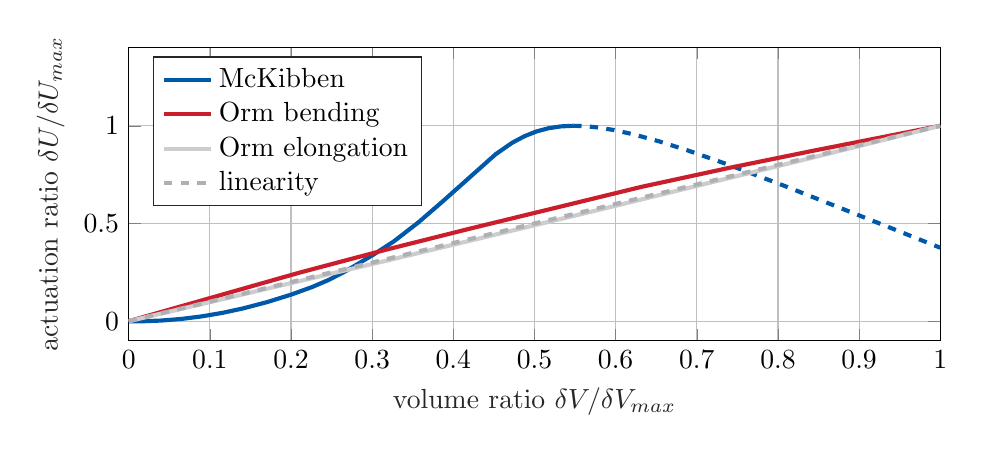
\begin{tikzpicture}

\begin{axis}[%
width=0.85\textwidth,
height=0.307\textwidth,
at={(0\textwidth,0\textwidth)},
scale only axis,
xmin=0,
xmax=1,
xlabel style={font=\color{white!15!black}},
xlabel={volume ratio $\delta V/\delta V_{max}$},
ymin=-0.1,
ymax=1.4,
ylabel style={font=\color{white!15!black}},
ylabel={actuation ratio $\delta U/\delta U_{max}$},
axis background/.style={fill=white},
xmajorgrids,
ymajorgrids,
legend style={at={(0.03,0.97)}, anchor=north west, legend cell align=left, align=left, draw=white!15!black}
]
\addplot [color=mycolor1, line width=1.5pt]
  table[row sep=crcr]{%
0	6.64468480238156e-13\\
0.0201005025125628	8.75243204948584e-05\\
0.0402010050251256	0.00332512405897667\\
0.0653266331658292	0.0117331904478247\\
0.0904522613065327	0.0249046492743175\\
0.115577889447236	0.0427513892029003\\
0.14070351758794	0.0651852988980188\\
0.170854271356784	0.0980369938635274\\
0.201005025125628	0.137215076581811\\
0.226130653266332	0.175068238130177\\
0.246231155778895	0.210907579628632\\
0.266331658291457	0.253741729445041\\
0.301507537688442	0.340391220232792\\
0.326633165829146	0.408312170236871\\
0.35678391959799	0.505004911261358\\
0.386934673366834	0.613214975063938\\
0.452261306532663	0.854807008382492\\
0.472361809045226	0.912631277406958\\
0.487437185929648	0.94626403813337\\
0.50251256281407	0.971128058957608\\
0.517587939698492	0.987706878146325\\
0.532663316582915	0.996954723086223\\
0.547738693467337	0.99999221332643\\
};
\addlegendentry{McKibben}

\addplot [color=mycolor1, dashed, line width=1.5pt, forget plot]
  table[row sep=crcr]{%
0.547738693467337	0.999992213326431\\
0.562814070351759	0.997904288874742\\
0.577889447236181	0.99164328364501\\
0.597989949748744	0.978152194257708\\
0.623115577889447	0.955019458927197\\
0.653266331658292	0.920692312660485\\
0.688442211055276	0.874489150713142\\
0.738693467336683	0.801248259588044\\
0.809045226130653	0.690772107576309\\
0.92964824120603	0.492665242848079\\
1	0.375832322559426\\
};
\addplot [color=mycolor2, line width=1.5pt]
  table[row sep=crcr]{%
0	0\\
0.210526315789474	0.248560359457172\\
0.315789473684211	0.364483047571436\\
0.421052631578947	0.474225435476816\\
0.526315789473684	0.580610711535574\\
0.631578947368421	0.687207531094921\\
0.736842105263158	0.781882023858429\\
0.842105263157895	0.871079842203232\\
1	1\\
};
\addlegendentry{Orm bending}

\addplot [color=mycolor3, line width=1.5pt]
  table[row sep=crcr]{%
0	0\\
0.315789473684211	0.307874524709858\\
0.578947368421053	0.569396702028871\\
0.842105263157895	0.836523467033735\\
1	1\\
};
\addlegendentry{Orm elongation}

\addplot [color=mycolor4, dashed, line width=1.5pt]
  table[row sep=crcr]{%
0	0\\
1	1\\
};
\addlegendentry{linearity}

\end{axis}
\end{tikzpicture}%
  %% This file was created by matlab2tikz.
%
%The latest updates can be retrieved from
%  http://www.mathworks.com/matlabcentral/fileexchange/22022-matlab2tikz-matlab2tikz
%where you can also make suggestions and rate matlab2tikz.
%
\definecolor{mycolor1}{rgb}{0.00000,0.34510,0.65882}%
\definecolor{mycolor2}{rgb}{0.79216,0.11765,0.17255}%
\definecolor{mycolor3}{rgb}{0.80392,0.80392,0.80392}%
%
\begin{tikzpicture}

\begin{axis}[%
width=0.598\textwidth,
height=0.198\textwidth,
at={(0\textwidth,0\textwidth)},
scale only axis,
axis on top,
xmin=0.5,
xmax=1968.5,
tick align=outside,
y dir=reverse,
ymin=0.5,
ymax=650.5,
axis line style={draw=none},
ticks=none
]
\addplot [forget plot] graphics [xmin=0.5, xmax=1968.5, ymin=0.5, ymax=650.5] {fig_bellow-1.png};
\end{axis}

\begin{axis}[%
width=0.297\textwidth,
height=0.192\textwidth,
at={(0.647\textwidth,0.003\textwidth)},
scale only axis,
xmin=0,
xmax=1.5,
xlabel style={font=\color{white!15!black}},
xlabel={pressure (kPa)},
ymin=-10,
ymax=48,
axis background/.style={fill=white},
xmajorgrids,
ymajorgrids,
legend style={at={(0.03,0.97)}, anchor=north west, legend columns=2, legend cell align=left, align=left, draw=white!15!black}
]
\addplot [color=mycolor1, line width=1.5pt]
  table[row sep=crcr]{%
0	0.65625\\
0.020003	0.607624587537979\\
0.0500075000000004	0.52090890773257\\
0.080012	0.424462799914457\\
0.1100165	0.319525122884924\\
0.1500225	0.16696555164601\\
0.1900285	0.000453843840724666\\
0.2300345	-0.179454447130303\\
0.2700405	-0.372153366810661\\
0.320048	-0.630001243232804\\
0.370055499999999	-0.905382412366595\\
0.420063	-1.19674388884769\\
0.480072	-1.56508083669635\\
0.5500825	-2.0165425356607\\
0.6300945	-2.55434051746948\\
0.7501125	-3.38535698180596\\
0.8901335	-4.35081772356119\\
0.960144	-4.81451037470239\\
1.020153	-5.19385040983376\\
1.0701605	-5.4932991768767\\
1.120168	-5.77439258543766\\
1.160174	-5.98401481409548\\
1.20018	-6.1783911802236\\
1.240186	-6.35596306714165\\
1.2701905	-6.47717906047022\\
1.300195	-6.58741633640641\\
1.3301995	-6.68602721835403\\
1.360204	-6.77236958167331\\
1.380207	-6.82280123133512\\
1.40021	-6.86731129683065\\
1.420213	-6.90571514194689\\
1.440216	-6.93782999961751\\
1.460219	-6.96347512113601\\
1.480222	-6.9824719229832\\
1.4999985	-6.99455975856444\\
};
\addlegendentry{volume}

\addplot [color=mycolor2, line width=1.5pt]
  table[row sep=crcr]{%
0	0\\
0.0100015000000013	0.00245869043011382\\
0.0200029999999991	0.0107835674422319\\
0.0300045000000004	0.0255780632427971\\
0.0400060000000018	0.0469985154368366\\
0.0500074999999995	0.0750519434101307\\
0.0600090000000009	0.109696367581613\\
0.0700104999999986	0.150875949865192\\
0.0900135000000013	0.252608954794749\\
0.1100165	0.37979748383194\\
0.1300195	0.531998503555851\\
0.150022499999999	0.708765607964072\\
0.170025500000001	0.909640085412999\\
0.1900285	1.13414697588932\\
0.220033000000001	1.51413512036515\\
0.250037500000001	1.94444209105579\\
0.280041999999998	2.42323219508909\\
0.310046499999999	2.94857465191582\\
0.340050999999999	3.51844359501607\\
0.380057000000001	4.34385328503755\\
0.420062999999999	5.23935282068943\\
0.460069000000001	6.19936000334119\\
0.5100765	7.4811093003182\\
0.560084	8.84236253474872\\
0.620093000000001	10.5627945055091\\
0.690103499999999	12.6602720193967\\
0.80012	16.061668942648\\
0.920137999999998	19.7501049078935\\
0.9901485	21.8053501323974\\
1.040156	23.1979116199186\\
1.0901635	24.5083250390544\\
1.1301695	25.486002185696\\
1.1701755	26.3913519495194\\
1.20018	27.0176133965181\\
1.2301845	27.5945524051951\\
1.260189	28.1184893518037\\
1.2901935	28.5857667374872\\
1.320198	28.9927551662133\\
1.340201	29.228809857066\\
1.360204	29.435415023046\\
1.380207	29.6115236392803\\
1.40021	29.7560980871467\\
1.420213	29.8681109002657\\
1.4302145	29.9115885676228\\
1.440216	29.9465454992476\\
1.4502175	29.9728564423065\\
1.460219	29.9903969139453\\
1.4702205	29.9990432230891\\
1.4902235	30\\
1.4999985	30\\
};
\addlegendentry{$\delta\text{ \!\!L}$}

\end{axis}

\begin{axis}[%
width=1.061\textwidth,
height=0.239\textwidth,
at={(-0.005\textwidth,-0.021\textwidth)},
scale only axis,
xmin=0,
xmax=1,
ymin=0,
ymax=1,
axis line style={draw=none},
ticks=none,
axis x line*=bottom,
axis y line*=left
]
\draw[-{Stealth}, color=mycolor3, line width=1.0pt] (axis cs:0.06,0.03) -- (axis cs:0.55,0.03);
\node[below right, align=left, font=\color{mycolor3}]
at (rel axis cs:0,0.11) {\scriptsize time};
\end{axis}
\end{tikzpicture}%
  \fi
  %\vspace{-6mm}
  \caption{}
\end{figure}
%
\clearpage
}

\newpage
% \begin{figure}[t]
% \centering
% \includegraphics[width=0.98\textwidth]{./3_chapters/0_introduction/img/modern_softrobots.png}
% \caption{\textit{a)} Elepant-inspired trunk [14]. \textit{b)}, Fish-inspired aquatic robot [19]. \textit{c)}, Soft-infalatable human robot arm [13]. \textit{d)}, Concentric-tube hard continuum robot[21]. \textit{e)}, Soft quadruped robot [20]. \textit{f)}. Explosion- driven semi-soft 3D printed robot [22]. }
% \end{figure}

% Perhaps a subtle point in the terminology above, is its mention to biology.
% Although the area of soft robotics has grown exponentially since the early 2010's, the field of soft robotics dates back to the early 60's.

% \begin{figure}
% \centering
% \setlength\figurewidth{0.53\textwidth}
% \setlength\figureheight{0.25\textwidth}
% \input{./3_chapters/0_introduction/img/myfigure.tikz}
% \end{figure}

%\subsection{REF}

The first robotic manipulator arm used in the orbital environment was the Space Shuttle remote manipulator system. It was successfully demonstrated in the STS-2 mission in 1981 and is still operational today.

First soft robot: Victor Scheinman and Larry Leifer developed an air-powered robot arm called Orm, which is the Norwegian word for snake.

% \begin{itemize}
%   \item . F. Shulte, "The Characteristics of the Mckibben Artificial Muscle", The Application of External Power in Prosthetics and Orthetics, pp. 94-115, 1960.
%   \item A. Chen, R. Yin, L. Cao, C. Yuan, H. K. Ding and W. J. Zhang, "Soft robotics: Definition and research issues," 2017 24th International Conference on Mechatronics and Machine Vision in Practice (M2VIP), 2017, pp. 366-370, doi: 10.1109/M2VIP.2017.8267170.
%   \item  W. C. R\"{o}ntgen, “Ueber die durch Electricität bewirkten Form—und Volumenänderungen von dielectrischen Körpern,” Ann Phys Chem, no. 11, pp. 771-786, 1880.
% \end{itemize}


(\textbf{Soft robotics in academia})
